\documentclass[10pt]{article}

\usepackage{ucs}
\usepackage[utf8x]{inputenc}
\usepackage[english]{babel}
\usepackage{fontenc}
\usepackage{graphicx}

\usepackage[dvips]{hyperref}

\author{Carson Holgate}
\title{Adiabatic Quantum Computation\\ at D-Wave Systems Inc.}
\date{05/10/2010}

\begin{document}
\maketitle

\paragraph{Adiabatic Quantum Computation}

as the name implies--relies on the adiabatic theorem to make computations. In 1928 Max Born and Vladimir Fock stated the theorem as follows: 
  \begin{quote}
   A physical system remains in its instantaneous eigenstate if a given perturbation is acting on it slowly enough and if there is a gap between the eigenvalue and the rest of the Hamiltonian's spectrum.
  \end{quote}
As it applies to quantum computation, if a non-degnerate system is initialized in the ground state 
  \[|\psi(0)\rangle\] 
of a given Hamiltonian 
  \[\mathcal{H}(0)\] 
and is allowed to evolve slowly according to the Schr\"{o}dinger equation 
  \[ i \frac{d}{dt} |\psi(t)\rangle = \mathcal{H}(t)|\psi(t)\rangle\] 
then as long as there is a non-zero energy gap between \(|\psi(0)\rangle\) and the next lowest energy state, \(|\psi(t)\rangle\) will remain close to the ground state of \(\mathcal{H}(t)\) at any given time.

Because it relies on the evolution of the state of a system, adiabatic quantum computation does not involve gates.   Instead, the solution to a given problem is encoded in the ground state of a problem Hamiltonain 
  \[\mathcal{H}_P\] 
It is generally easy to find \(\mathcal{H}_P\) but difficult to find the ground state. To complete the system an initial Hamiltonian 
  \[\mathcal{H}_B\] 
with an easily solveable ground state is chosen.  The system is described by both Hamiltonians as:  
  \[\mathcal{H}(t) = (1-t/T)\mathcal{H}_B + (t/T)\mathcal{H}_P\] 
Where T is a parameter to control the rate at which \(\mathcal{H}(t)\) varies.  Normalized to \(\tilde{\mathcal{H}}(s), 0 \leq s\leq 1\): 
  \[\tilde{\mathcal{H}}(s) = (1-s)\mathcal{H}_B + s\mathcal{H}_P\]
At this point the system is initialized to the ground state \(|\psi(0)\rangle\) where 
  \[\tilde{\mathcal{H}}(0) = \mathcal{H}_B\] 
and after sufficient time evolution \(|\psi(t)\rangle\) becomes the ground state of \(\mathcal{H}_P\)

\paragraph{D-Wave}
is the first company to develop a functional adiabatic quantum computer.  It was founded in 1999 by: 
  \begin{itemize}
   \item Haig Farris
   \item Geordie Rose (CTO)
   \item Bob Wiens (former CFO)
   \item Alexandre Zagoskin (Chief Scientist)
  \end{itemize}
and was started as an off-shoot of the University of British Columbia funding academic research in quantum computing.  

The company was founded with the goal of finding a way--with existing fabrication techniques--to solve a specific set of NP hard problems known as Quandratic Unconstrained Binary Optimization (QUBO) problems which are common in pattern matching problems and machine learning applications.  QUBO problems are equivalent to finding the lowest energy states of the two dimensional classical Ising Hamiltonian: 
  \[\mathcal{H} = \displaystyle\sum\limits_{i}h_i\sigma_{zi} + \displaystyle\sum\limits_{ij}J_{ij}\sigma_{zi}\sigma_{zj}\]

D-Wave accomplished this with a Superconducting Quantum Interference Device (SQUID) based flux quibit system:
 \begin{center}
  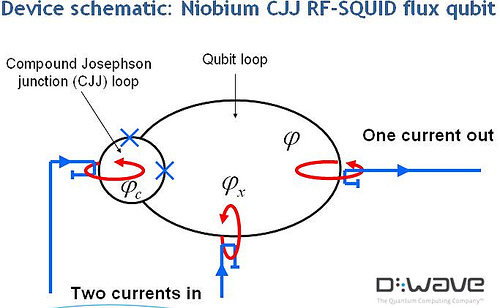
\includegraphics[scale=.7]{../img/Qubit_Schematic}
 \end{center}
which operates on low power at ultra low temperatures and has been manufactured at NASA's Jet Propultion Labratories.  

In 2007 D-Wave demonstrated example pattern matching Orion, thier 16-quibit system powered by the Chimera C4 chip.  Since then they have been working with Google on imaged based image search for applications like Google Goggles that makes use of vector matching and machine learning to recognize cars for vehicle safety systems.  D-Wave recently released early access to an API for Orion web services to allow users to submit programs to the quantum server.  Currently the web service backends to a server that simulates the Orion system but the actual quantum system should be up eventually.


\end{document}

